\documentclass{article}
\usepackage[english]{babel}
\usepackage{url}
\usepackage{graphicx}
\usepackage{amsthm}
\begin{document}
	\begin{titlepage}
		\centering
		{\scshape\Large INF142 submission one.\par}
		\vspace{3em}
		{{\scshape\large By Kristian Os \par}}
        \vspace{5em}
        
\includegraphics[scale=0.5]{uibLogo}
		\vfill
		\large\today
	\end{titlepage}
	\pagebreak
	\section{DNSSEC}
		\subsection{Definitions}
        \begin{itemize}
            \item DNS - is an abbreviation for Domain Name System
            \item DNSSEC - for Domain Name System Security Extensions.
            \item Root zone - This is the first node, DNS looks in the DNS hierarchy
            \item ZSK - Composed of a public key and a private key. Used to sign the fields in the area\cite{ovh}
            \item KSK - Composed of a public key and a private key. Used to sign the ZSK keys.\cite{ovh}
			\item ccTLD - Country code top-level domain, E.g .no, .se, .uk. 
            \item gTLD - Generic top-level domain.
        \end{itemize}
		\subsection{What does DNS do?}
		To reach another node on the Internet there must be denoted a number/name as an address. It must be unique so that one address only can point to one node.\\
		ICANN manages these so that each node has one of these unique addresses. For the same reason as we do not reference our devices based on their MAC-addresses, DNS translates the name version of the address to a number. This makes it much easier to remember the different number versions of the address.
		\subsection{Security}
		Within the DNS there are no security measures that can stand to the modern attacks that are getting more complex and malicious by the day. Recently a vulnerabilities in the DNS were found that allowed an attacker to redirect a DNS lookup to retrieve a false IP-address. This way the user gets a fake version of the intended site and the attacker can steal information or manipulate messages/transactions for their own gain.
	        \subsubsection{vulnerability? (Before DNSSEC)}
	        One DNS variant is DNS cache poisoning. For this exploit to work the attacker must get control of a DNS server and a DNS lookup must go through the poisoned DNS server. The attacker points an address like "www.uib.no" to a malicious IP-address. This way when a user types in "www.uib.no" he gets redirected to the malicious version of the site that the attacker owns.\cite{bellovin}
	        \subsubsection{After the implementation of DNSSEC}
	        With the implementation of DNSSEC organisations like UIB, Google and even the big tech leaders that controls the big nodes can sign the DNS records using public-key cryptography\cite{icann}
	        Now that each DNS server is signed with one of these keys the browsers know when a server is compromised and can select another one that is trusted.\\
	        \begin{figure}[ht]
	        	\centering
	        	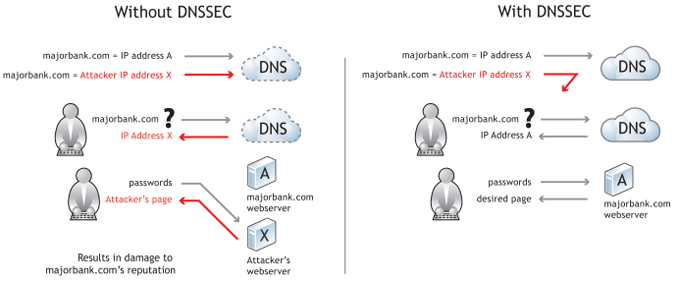
\includegraphics[width=1.0\textwidth]{dnsVsDnssec}
	        	\caption{Demonstrating DNSSEC on a theoretical plane.\cite{IcannDnssec}}
	        	\label{normal_case}
	        \end{figure}
				\paragraph{Keys - KSK and ZSK}
				KSK is a long term key and ZSK is a short term key. For the root zone these keys are generated at different intervals. These events are called "Root KSK Ceremonies" and here the KSK is used to sign a set of ZSKs that will be used to sign the DNS root zone for three months until the next new ceremony. \cite{iana}
		\subsection{A brief history of DNS and DNSSEC}  
		DNS was not implemented until a computer scientist Paul Mockapetris started the first DNS server in 1983. Before then everyone had to remember the relative IP-addresses which of course was very inconvenient and hard to do if you needed to keep track of many sites.
		It became an internet standard in 1986 and eventually caught on in the year 1988.
		This worked very well for two years until a computer scientist named Steven Bellovin discovered a major flaw in the DNS protocol. It was actually made a secret until 1995 when Internet Engineering Task Force(IETF) begins discussing implementation of a security addition to DNS.
		The fist capable version of DNSSEC was finished in 1999, but with a lot of remodelling and tests, the version that stood finished for zone implementation was done.
		The first zone to enable DNSSEC was Sweden, making .SE the first ccTLD to enable DNSSEC in march 2005.\cite{NLnetLabs}
		\subsection{In debt development of the DNSSEC}
		Discussing from the point Sweden implemented DNSSEC into their ccTLD to date the technology has gone through a lot. In 2007 Automated updates of DNS security Trust Anchors was implemented.\cite{trustAnchor} 
		Before this it the DNSSEC signatures normally came from the operating system or other trusted sources. Now it was possible to\cite{icann}
		
            
        
        
        
        
    
	\clearpage
	\section{Two-factor authentication}
		\subsection{Definition}
        
    \clearpage
	\nocite{*}
	\bibliography{mainBib}
	\bibliographystyle{plain}

\end{document}